% #############################################################################
% This is Chapter 4
% !TEX root = ../main.tex
% #############################################################################
% Change the Name of the Chapter i the following line
\fancychapter{End-to-End children automatic speech recognition}
\label{chap:e2e}
\cleardoublepage
\section{Introduction}
\label{chap:implement}
% End2End better and better
With the growing popularity of deep learning, numerous successful attempts to apply it to ASR have been made. It was only recently, that end-to-end models have shown their capability to outperform hybrid HMM-DNN systems for a variety of speech recognition tasks, including children's ASR. The major advantage of end-to-end speech recognition systems is the merging of the whole training process into a single neural network that eliminates the possibility of behavioural incompatibilities between modules that have been trained independently. However, because of the problem of children's data scarcity, the application of the end-to-end paradigm for children's ASR is relatively new and has not been extensively investigated \cite{gelin2021endtoend,sri_end2end,chen2020data,ng2020cuhk}. In addition, end-to-end models often require more parameters to provide such robustness and flexibility. As a result, training on small datasets becomes increasingly difficult \cite{luscher2019rwth}.

With the recent increased interest in end-to-end speech recognition, several architectures have been developed, including recurrent neural networks \cite{soltau2016neural} and neural transducers \cite{battenberg2017exploring}. However, one architecture stands out and consistently provides state-of-the-art results in large-vocabulary speech recognition for both adults and children, the Transformer.

This section dives more into details of the Transformer design as well as the adapter transfer for children ASR, a  parameter-efficient transfer for Transformer models that we have recently proposed.
\section{Transformer models}
\label{sec:trans_archi}

\begin{figure}[ht]
    \centering
    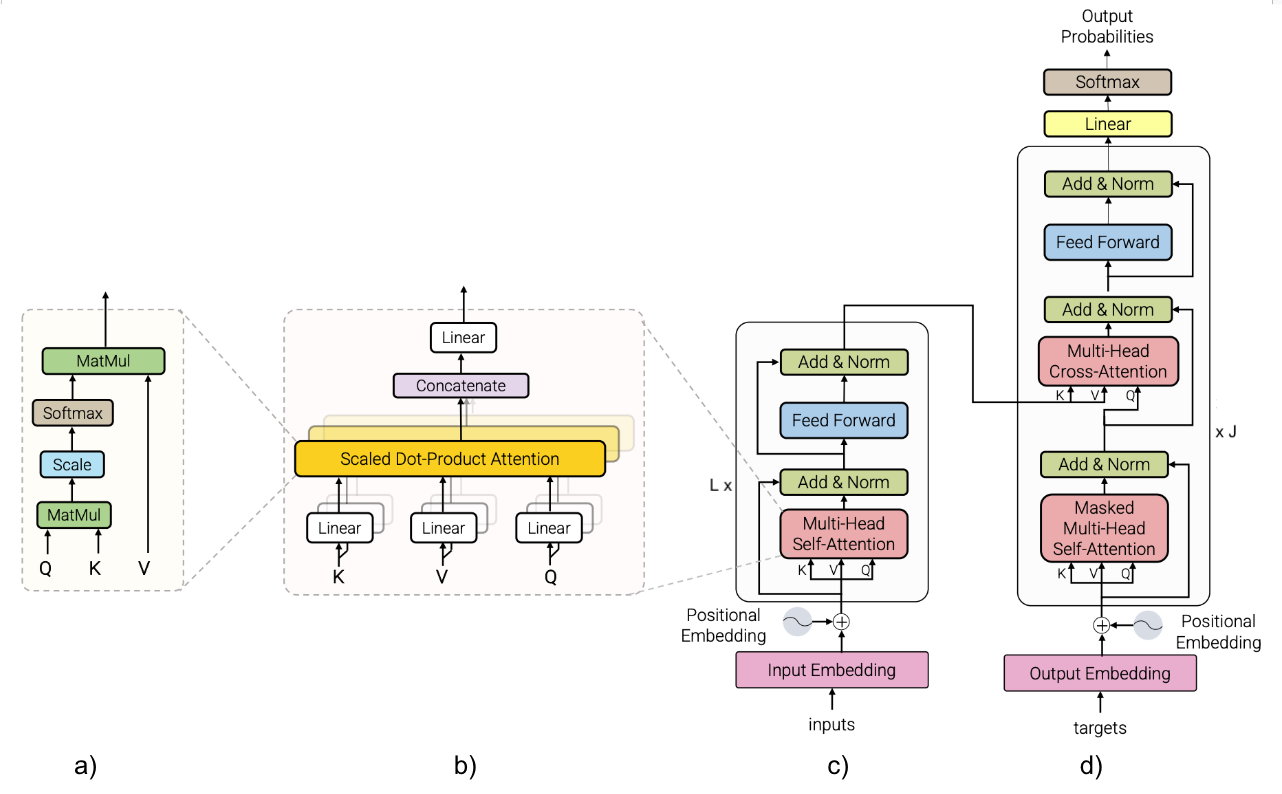
\includegraphics[width=1\textwidth]{imgs/transformer_archi.png}
    \caption{Architecture of the standard Transformer \cite{vaswani2017attention}. a) scaled dot-product attention, b) multi-head self-attention, c) Transformer-encoder, d) Transformer-decoder.}
    \label{fig:transformer_archi}
\end{figure}
% Explain transformer
First proposed in 2017 \cite{vaswani2017attention}, the Transformer architecture is a sequence-to-sequence encoder-decoder architecture that relies entirely on self-attention, eliminating recurrence, convolutions entirely and vanishing gradient issues. Another notable difference with recurrent neural networks is that the Transformer computes the dependencies between each pair of positions simultaneously, rather than one by one, by encoding the symbol position in the sequence. This, enables more parallelisation, resulting in faster training. Since its release, the Transformer architecture had tremendous impact in various areas, including NLP \cite{Bert}, computer vision \cite{dosovitskiy2020image}, and speech \cite{dong2018speech}.
The transformer encoder-decoder architecture is presented in figure \ref{fig:transformer_archi}, with c) the encoder and d) the decoder. The encoder's role is to transform an input sequence $X = x_1, \dots,x_T$ into a series of continuous representations $Z = z_1, \dots,z_T$ which are then fed into a decoder. The decoder, constructs an output sequence $Y = y_1, \dots, y_N$, one element at a time. At each time step, the decoder receives the encoder outputs together with the last decoder output, in an auto-regressive manner.

The information about the relative position of the tokens in the sequence is given by the summation between the input/output embedding and the positional embedding. Although there are many choices of positional encodings, \cite{vaswani2017attention} proposed to use sine and cosine of different frequencies as follows:
\begin{align}
    PosEnc_{(pos,2i)} = \sin(pos/10000^{2i/d_{\text{model}}})\\
    PosEnc_{(pos,2i+1)} = \cos(pos/10000^{2i/d_{\text{model}}})
\end{align}
Where $pos$ is the current token or label position and $i$ is the dimension.

The encoder is composed of a stack of N identical Transformer layers. Each layer consists of a multi-head self-attention module and a feed-forward fully connected neural network module. Each of these modules are followed by a normalization with a residual connection.
A multi-head self-attention (MHA) modules relies on the scaled dot-product attention \cite{vaswani2017attention}, illustrated in figure \ref{fig:transformer_archi}.a). Scale dot-product attention focuses on how relevant a particular token is with respect to other tokens in the sequence. And is defined as follows:
\begin{align}
    \text{Attention}(Q,K,V) = \text{softmax}(\frac{QK^T}{\sqrt{d_k}})V
    \label{equation:attention}
\end{align}
Where the input consists of queries Q, keys K of dimension $d_k$ and values V of dimension $d_v$. The dot product of the query with all keys is each divided by $\sqrt{d_k}$, then passes through a softmax function to obtain attention weights on the values. When $d_k$ is large, the scaling  $\frac{1}{\sqrt{d_k}}$ restrains the dot product from growing large in magnitude.

Instead of performing a single scaled dot-product attention, the MHA module linearly projects $h$ times K, V and Q with different, learned, linear projections to dimensions $d_k$,$d_k$ and $d_v$ respectively. On each of $h$ projected versions is performed the attention function \ref{equation:attention} in parallel. The output of each of the $h$ attention function, of dimension $d_v$ is concatenated and projected one last time as pictured in figure \ref{fig:transformer_archi}.b). More formally:
\begin{align}
    \text{MultiHead}(Q,K,V) = \text{Concat}(\text{head}_1, \dots, \text{head}_h)W^O \\
    \text{where } head_i = \text{Attention}(QW_i^Q, KW_i^K, VW_i^V)   \nonumber
\end{align}
Where the different projections matrices are $W_i^Q \in \mathbb{R}^{d_{\text{model}}\times d_k}$, $W_i^K \in \mathbb{R}^{d_{\text{model}}\times d_k}$, $W_i^V \in \mathbb{R}^{d_{\text{model}}\times d_v}$ and $W^O \in \mathbb{R}^{hd_{v}\times d_{model}}$.


In comparison to the encoder, the decoder contains a third sub-layer, which performs MHA over the output of the encoder using the prior sub-layer of the decoder as the query. The decoder's inputs, which are targets during training and the previously decoded label during inference, are offset by one position. This combined with a modified MHA prevents the attention to use subsequent positions, ensuring that the prediction at time-step $i$ solely depends on the previous $< i$ time-steps.

\section{Adapters for Transformer based models}

Age-dependent acoustic models have shown promising improvements, as children's age is highly correlated with acoustic variability \cite{children_language_model2, reviewASRchildren}. In particular, some studies found that variability decrease with the age, reaching the adult level at 15 years old \cite{Acoustic_change_children}.
%End2End and transfer learning
In parallel, research on End-to-end (E2E) architectures has shown equivalent or even superior performance in a large number of speech recognition tasks compared to traditional hidden Markov models approaches \cite{hmm-end2end}. E2E architectures propose to combine different modules of the ASR pipeline into a single deep neural network (DNN), resulting in benefits to avoid error accumulation and mismatch between components.
However, for these models to work properly, they need to be trained with a large amount of data, which is not commonly available for children's speech. Thus, to overcome children's data sparsity issue for E2E models training, \cite{sri_end2end,gelin2021endtoend} successfully used transfer learning by fine-tuning an adult pre-trained model on children's speech.
%Motivation for adapter

In this work, we propose to apply adapter modules on top of an adult acoustic model as an alternative to the transfer learning strategy for automatic children's speech recognition. Adapters are a method recently proposed for Transformer-based systems that consist of a small set of additional layers that are attached to a source model \cite{houlsby,pfeiffer}. Adapters are typically less expensive both in terms of training speed and storage cost, which is a desirable property in the case of aiming at the development of children's age-dependent models.  In addition, adapters overcome the problem of catastrophic forgetting. Indeed, after using transfer learning, the source model is completely overwritten by the newly trained weights, leading to a drop of performance on the source task. Whereas in adapter transfer, the backbone model remains frozen, thus preserved if adapter layers are removed. Adapters are therefore very practical in the context of small device computing where it can be expensive to load and store a large number of models for adults and children of different ages. Finally, in this work, we also propose a novel version of adapter layers inspired by variational auto-encoders (VAE)\cite{VAE}, so-called variational adapters or Vadapters. We hypothesize that the ability of VAEs to estimate variability can be applied in adapters to make them more suitable for parameter-efficient automatic children's speech recognition.



 %The structure of this work is organized as follows. Section \ref{section:SOA} reviews end-to-end ASR and adapters. In Section \ref{Vadapters}, we introduce our Vadapter architecture for children adapter transfer. The experimental setup is described in Section \ref{section:methods}. Section \ref{section:exp} presents  experimental results for the different adapter architectures. Finally, in Section \ref{section:conclusions} we conclude this paper and present potential perspectives for future work.


\subsection{Related work}
\label{section:SOA}
\subsubsection{Transformer model for children ASR}
% Motivation children E2E
Recently, E2E-based ASR models have demonstrated their ability to achieve state-of-the-art performance on a wide variety of speech recognition tasks \cite{hmm-end2end}. This fact motivated the assessment and comparison of different E2E architectures for children ASR \cite{sri_end2end,gelin2021endtoend}. These works found that Transformer-based architectures, described in the previous section \ref{sec:trans_archi}, yield the best results when an adult pre-trained model is fine-tuned for children using transfer learning with the help of the joint attention and CTC objectives \cite{First_End2End}. Usually, these two objectives are combined  as follows:
% Transformer 
%Transformers were first introduced in Natural Language Processing (NLP) for machine translation task \cite{vaswani2017attention}. Due to its success, it has been used in many other areas such as computer vision \cite{VIT}, language understanding \cite{Bert} and speech  \cite{dong2018speech}. Transformer is a neural sequence transducer based on an encoder-decoder architecture that relies solely on attention mechanism. Acoustic features are given to the encoder that maps them into a high-level representation. The encoder output is then fed to the decoder that predicts tokens, usually characters. As showed by \cite{gelin2021endtoend}, the best way to train and infer children's speech by using Transformer is by jointly using the attention objective with a Connectionist Temporal Classification (CTC) objective \cite{First_End2End}. Usually, attention and CTC objectives are combined  as follows:
\begin{equation} \label{equa:loss_asr}
    \mathcal{L}_{ASR} = \lambda_{ctc} \mathcal{L}_{ctc} + (1- \lambda_{ctc})\mathcal{L}_{s2s}
\end{equation}
where $\mathcal{L}_{ctc}$ and $\mathcal{L}_{s2s}$ are the CTC and attention losses, respectively. A hyper-parameter $\lambda_{ctc} \in [0,1]$ is used to control contribution of each loss. 
\subsubsection{Adapters}
\begin{figure}[t]
\begin{center}
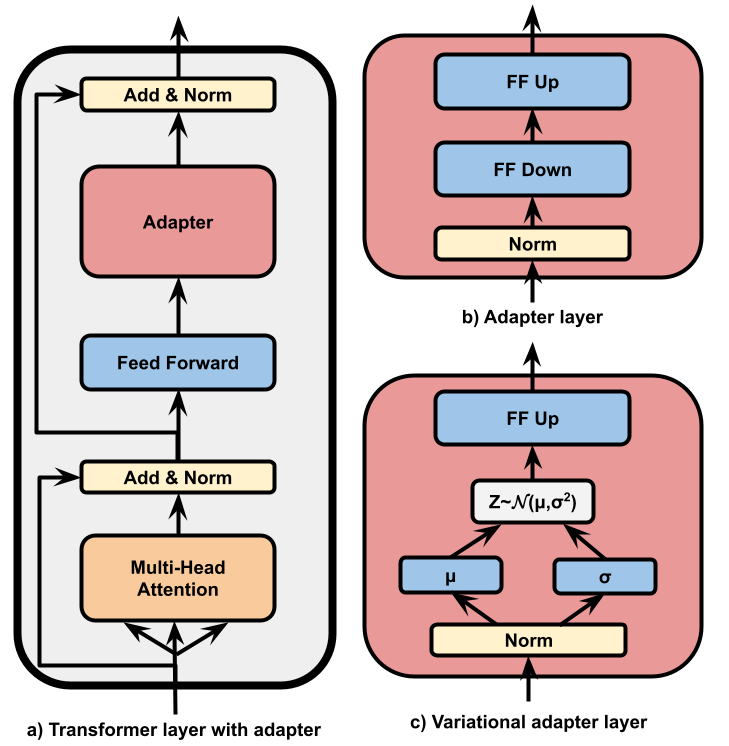
\includegraphics[scale=0.3]{imgs/Adapters.png}
\caption{a) Example of a Transformer layer with an adapter layer (adapted from \cite{pfeiffer}); b) Adapter layer; c) Vadapter layer}
\label{fig:all}
\end{center}
\end{figure}

% Adapters
Adapters were first introduced in the NLP field, motivated by the need for a parameter-efficient adaptation to fine-tune large models, like Transformer, on various text classification tasks \cite{houlsby}. They are a simple alternative to full model fine-tuning, as they involve only a small number of newly inserted parameters at each layer of the transformer.
While different positions have been proposed \cite{houlsby,pfeiffer}, they are generally plugged after the feed-forward layer (see Figure \ref{fig:all}.a). The key idea for training adapters is to freeze the backbone model's parameters and only update the adapter's parameters. Adapter modules are based on a bottleneck architecture (projection-down followed by a projection-up) as shown in Figure \ref{fig:all}.b.  Adapters solve a number of drawbacks associated with full model fine-tuning, such as parameter efficiency, faster learning iterations and a highly modular design

Since it was first proposed, adapters have been successfully used in a wide range of NLP tasks such as language understanding \cite{pfeiffer} and neural machine translation \cite{philip2020monolingual}. Some researchers proposed to use adapters for ASR tasks, such as in multilingual ASR \cite{kannan2019large}. More recently, \cite{tomanek2021residual} studied adapters for atypical speech, in particular pathological and accented speech. More recently, \cite{fan2022draft} proposed to use adapters inside of self-supervised models for children ASR by refining the whole model together with the weights of the adapters. Our work differs because our aim is to update only the adapters' weights in order to keep both the parameter efficiency and modular properties of adapters.

\subsubsection{Variational Auto-Encoders}
Variational auto-encoders (VAE) \cite{VAE} are a probabilistic generative models, that has been successfully applied in different speech tasks such as transformation \cite{vae_transformation} and enhancement \cite{vae_enh}. The main strength of VAE is their ability to learn a smooth representation of the latent space. Indeed, rather than producing a single value to describe each element of the latent space, as a standard auto-encoder, VAE provides a probability distribution: 
\begin{equation}
    p_{\theta}(\vb{x},\vb{z}) =  p_{\theta}(\vb{x}|\vb{z}) p_{\theta}(\vb{z})
\end{equation}
where $\vb{x}$ is the observed data generated by a random process using latent data $\vb{z}$ and $\theta$ denotes the distribution parameters. In this model, the likelihood function $ p_{\theta}(\vb{x}|\vb{z})$ quantifies   how the generation of $\vb{x}$ is conditioned by $\vb{z}$, while the prior $p_{\theta}(\vb{z})$ is used to regularize the latent data $\vb{z}$. Typically, a standard Gaussian distribution is used for the prior distribution
\begin{equation}
    p_{\theta}(\vb{z}) = \mathcal{N}(\vb{z}; 0, I)
\end{equation}
while the likelihood is defined as a multivariate Gaussian distribution:
\begin{equation}
     p_{\theta}(\vb{x}|\vb{z}) = \mathcal{N}(\vb{x}; \mu_{\theta}(\vb{z}), \sigma^2_{\theta}(\vb{z}))
\end{equation}
where $\mu_{\theta}(\vb{z})$ and $\sigma^2_{\theta}(\vb{z})$ are obtained using $\vb{z}$. However, since the posterior distribution $p_{\theta}(\vb{x}| \vb{z})$ is intractable, it is approximated with the auxiliary distribution $q_{\phi}(\vb{z}| \vb{x})$ that plays the role of an encoder:
\begin{equation}
    q_{\phi}(\vb{z}|\vb{x})= \mathcal{N}(\vb{z}; \Tilde{\mu}_{\phi}(\vb{x}), \Tilde{\sigma}^2_{\phi}(\vb{x}))
\end{equation}
 We also want to ensure that the approximate posterior $q_{\phi}(\vb{z}|\vb{x})$ and the true posterior $ p_{\theta}(\vb{z}|\vb{x})$ are similar by minimizing the Kullback-Leibler (KL) divergence between the two distributions. 
\begin{equation} \label{equa:minKL}
     \min KL(q_{\phi}(\vb{z}|\vb{x})|| p_{\theta}(\vb{z}| \vb{x}))
\end{equation}
It is possible to minimize expression (\ref{equa:minKL}) by maximizing the following expression as shown in \cite{vae_transformation}:
\begin{equation}
    \mathbb{E}_{q_{\phi}(\vb{z}| \vb{x})} \log p_{\theta}(\vb{x}|\vb{z}) - KL(q_{\phi}(\vb{z}|\vb{x})|| p_{\theta}(\vb{z}))
\end{equation}
Where the first term is the reconstruction error and the second term a regularisation. %Generally, we choose $p_{\theta}$ to be a standard normal distribution $\mathcal{N}(0,1)$.

Thus, the VAE loss function can be define as followed:
\begin{align}
\mathcal{L}_{VAE} & = \mathcal{L}_{recons}+ \mathcal{L}_{KL} \\
                  & = \mathcal{L}_{recons}+ \sum_j KL((q_{\phi}^{(j)}(\vb{z}|\vb{x})|| p_{\theta}(\vb{z}))
\end{align}
for each dimension $j$ of the latent space. 

\subsection{Variational adapters}
\label{Vadapters}
% Motivation (latent space more continuous)
Adapters and auto-encoders (AE) share a similar encoder-decoder structure. Although the purpose of these two architectures is different, the role of their encoders is similar: map relevant characteristics of the input into a unique latent vector. On the other hand, their architecture differs in the decoders: AEs use the decoder to reconstruct the input, while adapters project the information contained in the latent vector to be processed by the next layer. Consequently, adapters suffer from the same problems as AEs, a poor capability to model variability.
In order to be more robust to the high variability of children's speech, we propose to represent each latent value in probabilistic terms. To this end, we propose Vadapter, a new adapter architecture in which the encoder structure of the adapter is replaced with the structure of a VAE's encoder as shown in Figure \ref{fig:all}.c.    

Consequently, during training, instead of a down-projection that maps the input into the latent representation, we now have two branches, producing the mean $\mu$ and variance $\sigma$. During inference, $\mu$ is used directly as a deterministic latent vector, discarding $\sigma$. We hypothesise that this deterministic inference allows Vadapters to capture variability in the $\sigma$ branch while keeping the $\mu$ more robust. In addition, dropping the $\sigma$ branch during inference keeps the number of parameters equivalent to normal adapters, thus preserving the parameter efficiency.

Similarly to VAEs, the regularisation term which ensures that the distribution of $q_{i}(\vb{z}| \vb{x})$ for each Vadapter at layer $i$ is similar to the standard normal distribution $p(\vb{z})$ is required. However, as there are many Vadapter layers we normalise the sum of all regularization terms by the number of Vadapter layers: 
\begin{equation}
    \mathcal{L}_{KL_{all}}  = \frac{\sum_L^iKL(q_{i}(\vb{z}|\vb{x})|| p(\vb{z}))}{L} \\
\end{equation}
where $L$ is the total number of Vadapters in the model. 
Then, we inject this regularisation loss into the E2E ASR loss defined in equation (\ref{equa:loss_asr}) as follows:
\begin{equation}\label{loss}
    \mathcal{L}_{ASR} = \lambda_{ctc} \mathcal{L}_{ctc} + (1- \lambda_{ctc})\mathcal{L}_{s2s}  + \beta \mathcal{L}_{KL_{all}} 
\end{equation}
where $\beta$ is an hyper-parameter to control the regularization's contribution.

\subsection{Experiments}
\label{section:methods}

\subsubsection{Corpus}
\begin{table}[ht]
\centering
\begin{tabular}{c|c|c}
\hline
 Training & Validation     & Test   \\ \hline
60897 utterances  & 10044 utterances   & 4079 utterances \\ 
 566 speakers  & 79 speakers   & 91 speakers \\ 
 113 hours  & 18 hours   & 13 hours \\ \hline

\end{tabular}
\caption{My Science Tutor Children Speech Corpus statistics}
\label{tab:statistics_myst}
\end{table}
In this work, we decided to use the Boulder Learning My Science Tutor (MyST) corpus, described in section \ref{section:children_corpora} given the task assigned to the children, which is to speak spontaneously. Indeed, the end-to-end model encapsulates the acoustic model and language model in the same network. As a result, if we train a model with a restricted amount of prompts on a data set of reading tasks, the model will learn and overfit the prompts. Thus, yielding unreliable results. Furthermore, for the purposes of our experiments, we decided to remove all utterances shorter than one second and longer than 20 seconds. . The details of the filtered corpora used in our work are presented in Table \ref{tab:statistics_myst}. 
\subsubsection{Implementation details}

% Model description
All experiments were performed using the SpeechBrain toolkit \cite{speechbrain}. We used  12 Transformer layers for the encoder and 6 Transformer layers for the decoder, all with dimensions 512. This model has been pre-trained using the LibriSpeech dataset\cite{librispeech} and is publicly available\footnote{https://huggingface.co/speechbrain/asr-transformer-transformerlm-librispeech}. Furthermore, for all of our experiments, we used the same Transformer language model, trained on 10 million words in order to only evaluate the contribution of the E2E model. The adapter architecture consists of a linear layer down-projection from dimension 512 to 256 with a ReLu activation, followed by a linear layer up-projection from dimension 256 back to 512. We analysed the influence of the latent dimension, i.e. the number of parameters, on the ASR performance in more detail in section \ref{section:exp}. The Vadapters $\sigma$ and $\mu$ branches consist of a linear layer down-projection from 512 to 256 each, while the up-projection remains the same as the aforementioned traditional adapters. For all the experiments,  models were trained with a batch size of 16, $\lambda_{ctc} = 0.3$ and the same decoding hyper-parameters.
All models were trained with a learning rate of 1.5e-4, for 40 epochs. Finally, for all our Vadapter experiments we choose $\beta = 1.0$.

\subsubsection{Experiments description}
In our first experiment, we will attempt to determine which component of the transformer model is most important to ASR children. As a result, this information will be used to determine the best location of the adapters in the transformer layer. Indeed, the adapter should come after the most important component since it will project the output of that component into the expected transformer space. In order to do this, we studied the role of each transformer layer sub-module by fine-tuning one or two of them with the children's speech data.


% Experiments description
Secondly, we analyze the performance of adapters in three scenarios: i) Adapters in all layers of the E2E model, ii) adapters only  present in the encoder layers, and iii) adapters only in the decoder layers. These experiments are motivated by the fact that the encoder is closely related to the acoustics generating a high-level representation of speech, while the decoder generates output tokens related to the linguistic domain. The objective is then to evaluate which components, the encoder  (acoustics) or the decoder (linguistics), benefit more from the adapter transfer.
In order to compare our new architecture with traditional adapters, we reproduce the three scenarios mentioned above by replacing the adapters with our Vadapters. Furthermore,  we evaluate the combination of Vadapter and traditional adapter in two scenarios, Vadaper in the encoder and adapter in the decoder, and vice versa.

\subsection{Results}
\label{section:exp}

\subsubsection{Transfer learning experiments}
\begin{table}[ht]
\centering
\begin{tabular}{lcc} \toprule
Fine-tuned part & WER $\downarrow$  & Trained parameters\\\hline
None & 25.04\% & - \\
Full model & 13.50\% & 71.5M\\ \hline
Norm & 18.08\% & 57.9K\\
MHA & 13.40\% & 25.2M \\
FFN & \textbf{12.57\%} & 37.8M \\ \hline
MHA + FFN & 12.78\%  & 63.0M\\
Norm + FFN & 12.92\% & 37.9M \\
Norm + MHA & 13.52\%  & 25.3M\\ \hline
\end{tabular}
\caption{Results of the fine-tuning on part of the model only}
\label{tab:result_TL_transformer}
\end{table}
Table \ref{tab:result_TL_transformer} shows results of the transfer learning on sub-modules of the Transformer model. Fine-tuning all the transformer's parameters, in the same way as the previous work \cite{sri_end2end,gelin2021endtoend}, gives better results than using the model trained only on adult data with 13.76\% compared to 25.04\% WER respectively. The fine-tuning of all normalisation weights improved the score compared to the adult model with 18.04\% but still under-perform compared to the full fine-tuning. Thus, the normalisation contribution in the children's transfer learning is limited. In contrast, fine-tuning the MHA or FFN yields better, results compared to the full transfer learning with 13.40\% and 12.57\% WER respectively. While always outperforming a full model update, the use of transfer learning on a combination of different model components reduces performance when compared to FFN alone. Transfer learning becomes more difficult by updating the weights of all components of the transformer as well as the non-transformer weights (i.e., Convolution blocks and embedding blocks), which explains why the entire fine-tuning produces worse results. In conclusion, FFN modules are the most relevant to fine-tune using transfer learning. This is because transformer feed-forward layers are key-value memories \cite{geva2020transformer}, where each key correlates with patterns in the training examples, and each value produces a distribution over the outputs. Consequently, adapters should be placed after the FFN sub-modules in order to achieve better results. This is consistent with Pfeiffer's work for NLP tasks \cite{pfeiffer}.

\subsection{Adapters and Vadapters results}
\begin{table}[t]
\begin{tabular}{ccc}
\hline
 Method & WER     & Trained parameters   \\ \hline
\multicolumn{1}{l}{No fine-tune} & 25.04\%   & - \\ 
\multicolumn{1}{l}{Fine-tune} & 13.50\% & 71.5M \\ \hline
\multicolumn{1}{l}{Adapter}  &   14.33\% & 4.8M  \\ 
\multicolumn{1}{l}{Adapter encoder only }    & 14.56\% & 3.2M  \\ 
\multicolumn{1}{l}{Adapter decoder only} & 20.10\%      & 1.6M  \\ \hline
\multicolumn{1}{l}{Vadapter} & 14.19\%     & 7.1M (4.8M)  \\
\multicolumn{1}{l}{Vadapter-enc + Adapter-dec } & 14.05\%     & 6.3M (4.8M)  \\
\multicolumn{1}{l}{Adapter-enc + Vadapter-dec } & 14.35\%     & 5.5M (4.8M)  \\
\multicolumn{1}{l}{Vadapter encoder only} & 14.51\%     & 4.7M (3.2M)  \\ 
\multicolumn{1}{l}{Vadapter decoder only} & 20.23\%     & 2.4M (1.6M)  \\ \hline

\end{tabular}

\caption{Results of the different approaches; In parenthesis are shown the number of parameters needed for inference after dropping the $\sigma$ branch.}
\label{tab:res}
\end{table}
\subsubsection{Adapters for children ASR}
Table \ref{tab:res} presents the word error rate (WER) results of the different approaches.
Firstly, the pre-trained Transformer adult model without any adaptation gives the worst result, with a WER of 25.04\%, while adult performances on Librispeech corpus are usually less than 6\%. 
This result shows the impact of the variability in child speech.
% ALBERTO: This result shows the impact of the variability in child speech. : DONE
Secondly, the adaptation of all 71.5 million parameters for children's speech resulted in a considerable improvement, with 13.50\% WER. This result correctly reflects the state-of-the-art performance obtained in the literature for the MyST corpus \cite{sri_end2end}. 
Regarding adapters, similarly to previous work in NLP \cite{houlsby} and ASR \cite{tomanek2021residual}, we observe that they perform slightly worse than fine-tuning, with a score of 14.33\% WER. However, it is important to note that adapters require less than 10\% of all parameters of the full fine-tuning. We also investigate adapter transfer for encoder and decoder only. Table \ref{tab:res} shows that adapters are more relevant when plugged into the encoder with 14.56\% WER while compared to the decoder with 20.10\% WER. This result confirms that acoustic variability plays a critical role in the degradation of children ASR performance \cite{shivakumar2020transfer}. 

Additionally, we also evaluated how different adapter hidden-dimension, i.e. the number of parameters, influence the speech recognition performance compared to the fine-tuning model.
Figure \ref{fig:ratio} displays the relative WER delta over the ratio of trainable parameters compared to the fine-tuned model. As a reference, the relative WER delta of the adult model with respect to fine-tuning is 85.5\%.
% ALBERTO: Add here: "As a reference, the relative WER delta of the adult model with respect to fine-tuning is 85.5\%.": Done
%We observe that the delta increases as the number of trainable parameters decreases.
We observe that the performance difference between fine-tuning and adapters decreases as the number of trainable parameters increases.
% ALBERTO: This observation is in reverse order of the Figure. I think it would be more clear so say: "We observe that the performance difference between fine-tuning and adapters decreases as the number of trainable parameters increases."
% ALBERTO: Can this figure show 2 constant lines? The fine-tuning performance and the adult model performance? Because this will allow saying something like: "While with only 2\% of the trainable parameters, adapters manage to surpass by a large margin the source model performance, adapters need a minimum amount of parameters to get close to the fine-tuning performance" Then, the 2 following sentences disappear and you would continue in "Nevertheless, ...": DONE
While with only 2\% of trainable parameters, adapters manage to surpass by a large margin the source model performance, adapters need a minimum amount of parameters to get close to the fine-tuning performance. Nevertheless, adapter transfer outperforms full fine-tuning, when the number of parameters used is around 30\% of the number of the entire model. There is therefore a trade-off between performance and parameter efficiency. A similar observation has been made in \cite{fan2022draft}.
%This degradation can be explained by the fact that in order to process children's speech, adapters need a certain amount of parameters. The model cannot be robust to children's speech variability when there are not enough parameters.

\begin{figure}[t]
\begin{center}
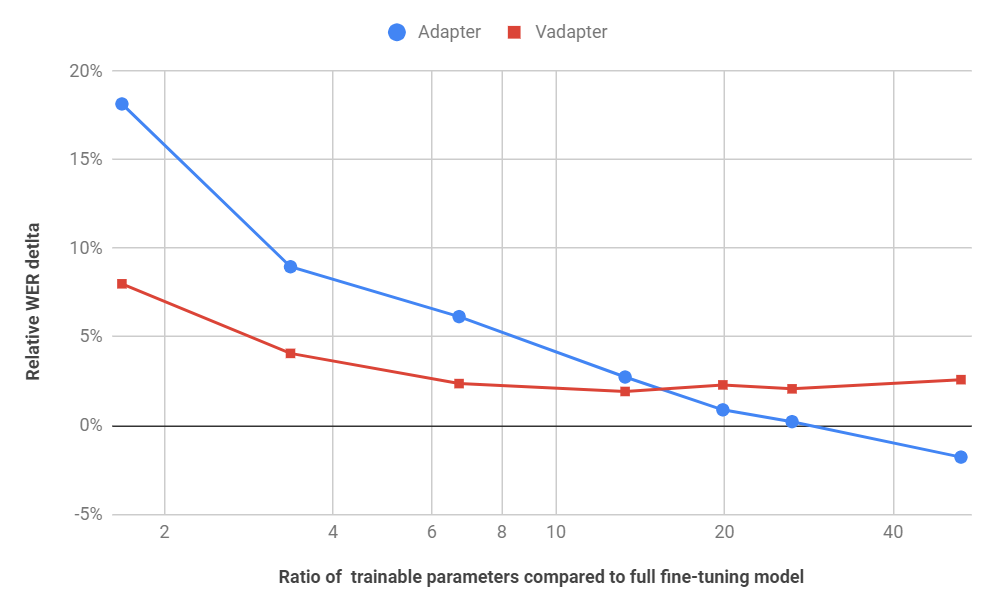
\includegraphics[scale=0.3]{imgs/ratio_delta.png}
\caption{Relative WER delta over the ratio (\%) of trainable parameters compared to full fine-tuned model.}
\label{fig:ratio}
\end{center}
\end{figure}
\vspace{-0.35cm}
\subsubsection{Variational-adapters}
Concerning the Vadapter architecture, with the exception of the cases where the Vadapters are placed in the decoder, all the scores are higher than their conventional counterpart, approaching the full fine-tuning score. The best configuration, Vadapter in the encoder and adapters in the decoder, reaches 14.05\% WER. In the same way, as for the conventional adapters, we can see that the Vadapters are more advantageous when placed in the encoder since the score is 14.51\% WER for Vadapters in the encoder only and 20.23\% WER for the decoder only. We believe that this is because Vadapters are designed to be more robust to acoustic variability, 
% ALBERTO: "We believe that this is because Vadapters...": Done
which is mainly present at the encoder level. Thus, the Vadapters in the decoder does not manage to improve the score of their conventional counterpart. 

Thus, we tested several possible combinations between Vadapter and adapters. We observe that the configurations with Vadapters in the encoder are giving the best results, with 14.19\% WER for Vadapters in both the encoder and the decoder, as well as 14.05\% for Vadapters in the encoder and adapters in the decoder. However, when Vadapters are placed in the decoder in combination with adapters in the encoder the result is not as good as adapters everywhere with 14.35\% WER. We believe again that this is due to the variability being more present in the acoustic than in the linguistic component.
% ALBERTO: "We believe again that this is due to ...: Done

Finally, as shown in Figure \ref{fig:ratio}, Vadapter outperforms conventional adapters when the number of parameters is less than 15\% of the full model. Indeed, the Vadapters are always under 10\% relative WER delta compared to full fine-tuning and reach under 5\% with less than 4\% of the ratio of trainable parameters, where conventional adapters start above 15\% relative WER delta and need more than 10\% of the ratio of trainable parameters to be under 5\% relative WER delta. These results confirm the proposed Vadapter architecture as a more convenient alternative for parameter-efficient transfer learning. However, when the number of parameters increases,  the results drop compared to conventional adapters. We hypothesize that this is due to the more complex and subject to variability sampling  of $\vb{z}$ during Vadapters training.


\subsection{Discusion}
\label{section:conclusions}
% Train age dependent variational-adapter and use AdapterFusion
In this work, we demonstrate the usefulness of adapter transfer in the context of children's speech. With less than 10\% of the total number of fine-tuning parameters, adapters are able to efficiently model children's speech. Noticeably, the adapter performance approaches fine-tuning, as the number of parameters increases. Furthermore, our Vadapter architecture outperforms conventional adapters in terms of acoustic variability robustness in a parameter-efficient setting. Using a combination of Vadapters in the encoder and conventional adapters in the decoder allows for further improvement, getting closer to the fine-tuning performance while keeping a small number of parameters.  This seems to demonstrate their effectiveness in modelling highly variable data, such as children's speech.
%This work is our first step towards the development age-dependent E2E ASR.
%In future work, we would like to train age-dependent adapters %and fuse them using attention.
%as well as investigate the behavior of new adapter architectures on children's speech.

\section{Summary}
We covered the state-of-the-art for end-to-end children's speech recognition in this chapter. Particularly, the usage of the Transformer architecture in conjunction with transfer learning. In a similar way as chapter \ref{chapter:Hybrid}, to avoid a drop in performances attributable to an acoustic mismatch between children and adults, the end-to-end model should be trained with children's data. In contrast to previous work, we demonstrated that fine-tuning only a portion of the transformer modules, particularly the FFN sub-module, yields better results since it serves as a key-value memory. As a result, we placed our adapter subsequent to it. The adapter's role is to accomplish knowledge transfer, which is related to transfer learning. Rather than updating the complete model's weights, we just tweak an extra module, hence fewer parameters. This adapter transfer achieves almost identical results as the entire model fine-tuning. In addition, adapters are useful in the context of customized models, where training and storing a whole model for each age group or each child can be expensive and time-consuming.

In addition, we proposed the variational adapter, a variant of the traditional adapter based on variational auto-encoders. Compared to the adapter, which takes a bottleneck encoder-decoder structure with a linear layer as encoder and a linear layer as decoder, the variational adapter's encoder consists of two branches, $\mu$ and $\sigma$. The outputs of these two branches are used as the mean and variance vector to sample the input of the decoder. By doing so, we enforce the adapter's input variability to be contained in the $\sigma$ branch. A branch which is suppressed during inference. As a result, we reduce input variability while maintaining the same size as standard adapters.